\chapter{Plataforma de Desarrollo}
\label{ch:PlataformaDesarrollo}

En este capıtulo vamos a describir con más detalle todo el software utilizado en la realización del proyecto: programas, plataformas, simuladores, etc. El sistema operativo elegido para desarrollar todo el proyecto ha sido Ubuntu 16.04. Ubuntu es un sistema operativo basado en Debian GNU/Linux y que se distribuye como software libre, el cual incluye su propio entorno de escritorio denominado Unity. El nombre de la distribución proviene del concepto zulú y xhosa de ubuntu, que significa “humanidad hacia otros” o “yo soy porque nosotros somos”. Debido a las similitudes entre los ideales de los proyectos GNU, Debian y en general el movimiento del software libre, y el movimiento sudafricano encabezado por el obispo Desmond Tutu \textit{Premio Nobel de la Paz en 1984} llamado Ubuntu, la compañía británica Canonical Ltd. decidió nombrarlo en honor a dicho movimiento. El eslogan de Ubuntu – “Linux para seres humanos” (en inglés “Linux for Human Beings”) – resume una de sus metas principales: hacer de Linux un sistema operativo más accesible y fácil de usar.

\section{GitHub}
\label{sec:plat_github}

GitHub\cite{github} es una plataforma de desarrollo colaborativo de software para alojar proyectos utilizando el sistema de control de versiones Git (\textit{Sección \ref{subsec:plat_git}}). Utiliza el framework Ruby on Rails por GitHub, Inc. (anteriormente conocida como Logical Awesome). Aloja tu repositorio de código de forma pública (o privada creando una cuenta de pago) y te brinda herramientas muy útiles para el trabajo en equipo dentro de un proyecto. GitHub facilita toda la infraestructura para trabajar en equipos distribuidos a través de una interfaz web. Incluso si no trabajas en equipo, si tienes una copia de tu código fuente en GitHub, tienes un backup de todo el proyecto completo. Ese backup incluye no sólo el código que tienes ahora sino también de todo el historial de modificaciones que el código ha sufrido desde el primer día. Esta copia la puedes recuperar en cualquier momento y continuar trabajando desde cualquier ordenador.

También permite contribuir a mejorar el software de los demás. Para poder alcanzar esta meta, GitHub provee de funcionalidades para hacer un \textit{fork} y solicitar \textit{pulls}. Realizar un \textit{fork} es simplemente clonar un repositorio ajeno (genera una copia en tu cuenta), y trabajar sobre el para eliminar algún bug, modificar cosas o añadir funcionalidades. Una vez realizadas tus modificaciones puedes enviar un \textit{pull} al dueño del proyecto, el cual podrá analizar los cambios que has realizado fácilmente, y si considera interesante tu contribución, combinarlo con el repositorio original.

En la actualidad, GitHub es mucho más que un servicio de alojamiento de código. Además de éste, se ofrecen varias herramientas útiles para el trabajo en equipo. Entre ellas, caben destacar:
\begin{itemize}
	\item Una wiki para el mantenimiento de las distintas versiones de las páginas.
	\item Un sistema de seguimiento de problemas que permiten a los miembros de tu equipo detallar un problema con tu software o una sugerencia que deseen hacer.
	\item Una herramienta de revisión de código, donde se pueden añadir anotaciones en cualquier punto de un fichero y debatir sobre determinados cambios realizados en un commit específico.
	\item Un visor de ramas donde se pueden comparar los progresos realizados en las distintas ramas de nuestro repositorio.
\end{itemize}

Para comenzar a usarlo sólo hay que crearse una cuenta gratuita y ya tendremos acceso a todas sus funcionalidades. Para crear un repositorio solo hay que seleccionar el botón “Create a New Repo”, de la barra de herramientas, habiendo entrado a GitHub con tu cuenta y rellenar los datos de nombre y descripción del repositorio.

Para utilizarlo desde el ordenador, GitHub nos ofrece una serie de comandos para introducir en la terminal. Los más usados son:

\begin{itemize}
	\item git init: Con este comando indicamos que vamos a iniciar un proyecto en la carpeta actual, y que lo queremos sincronizar y gestionar mediante GitHub.
	\item git add: Con este comando añadimos archivos a la siguiente versión o actualización del proyecto. Su hacemos \textit{git add --all} estamos indicando que queremos añadir todo dentro de la carpeta donde estamos: los archivos nuevos, los eliminados, los modificados, etc.
	\item git commit: Usamos este comando para añadir un mensaje a la versión o actualización o para indicar los cambios hechos. Una forma de usarlo sería \textit{git commit -m “comentario”}
	\item git pull: Este comando se usa para descargar la última versión del código del repositorio, por ejemplo: \textit{git pull origin master}
	\item git push: Este comando se usa para subir el código al repositorio, por ejemplo: \textit{git push origin master}
	\item git remote add origin: Este comando se usa para establecer cuál es el repositorio al que subir el código o del cual descargar la última versión, por ejemplo: \textit{git remote add origin -url del repositorio-}
\end{itemize}

Para colaborar en un proyecto ajeno simplemente basta con buscarlo dentro de los repositorios en su página web, y luego presionar el botón fork. Esto genera automaticamente una copia del mismo en tu perfil y te permite trabajar sobre esa copia, sin peligro para el autor de que hagas modificaciones en su código. Al terminar tus modificaciones, y hacer los \textit{push} que necesites, podrás presionar Pull Request para enviárselo al autor y que él decida si acepta las modificaciones.

\subsection{Git}
\label{subsec:plat_git}

Git\cite{git} es un software de control de versiones diseñado por Linus Torvalds pensando en la eficiencia y la confiabilidad del mantenimiento de versiones de aplicaciones cuando estas tienen un gran número de archivos de código fuente. Se trata de un sistema distribuido de control de código fuente o SCM \textit{(Source Code Management)}. Un SCM es una herramienta que nos resuelve una serie de problemas, como saber qué líneas de código han cambiado de una versión a otra, volver a una versión anterior de forma sencilla o saber quién ha cambiado qué partes del código entre otros. En este caso, Git nos aporta herramientas para:

\begin{itemize}
	\item Auditoría del código: saber quién ha tocado qué y cuándo
	\item Control sobre cómo ha cambiado nuestro proyecto con el paso del tiempo
	\item Volver hacia atrás de una forma rápida
	\item Control de versiones a través de etiquetas: versión 1.0, versión 1.0.1, versión 1.1, etc. Sabremos exactamente que había en cada una de ellas y las diferencias entre cualquiera de ellas dos
	\item Seguridad: todas las estructuras internas de datos están firmadas con SHA1. No se puede cambiar el código sin que nos enteremos
	\item Merging y branching extremadamente eficientes
	\item Mejora nuestra capacidad de trabajar en equipo
\end{itemize}



\section{Blender}
\label{sec:plat_blender}

Blender\cite{blender} es un software libre y gratuito de creación en 3D. Está diseñado para realizar tareas como modelado, iluminación, renderizado, animación y creación de gráficos tridimensionales, edición de vídeo y escultura y pintura digital. En Blender, además, se pueden desarrollar vídeo juegos ya que posee un motor de juegos interno. Actualmente es compatible con todas las versiones de Windows, Mac OS X, GNU/Linux (Incluyendo Android), Solaris, FreeBSD e IRIX. Su interfaz utiliza OpenGL\footnote{\url{https://www.opengl.org/}} (\textit{Open Graphics Library}) para proporcionar una experiencia consistente y de calidad.

Blender fue liberado al mundo bajo los términos de la Licencia Pública General de GNU v2 (GPL)\footnote{\url{https://www.gnu.org/licenses/old-licenses/gpl-2.0.html}}, y su desarrollo continúa conducido por un equipo de voluntarios procedentes de diversas partes del mundo y liderados por el creador de Blender, Ton Roosendaal. 

Se eligió este programa para realizar la edición 3D de mundos para Gazebo frente a alternativas como 3DSMax, Maya o XSI por diversos motivos: es más ligero que sus competidores; posee más herramientas de escultura 3D; la comunidad es muy activa y hay gran cantidad de información, tutoriales y soluciones disponibles; y es de distribución comercial libre y gratuita. 


\section{Simulador Gazebo}
\label{sec:plat_gazebo}

Gazebo\cite{gazebo} es un simulador 3D de robots para interiores y exteriores, con un motor de físicas y cinemáticas muy potente. Dispone de un conjunto de plugins que facilita la integración con ROS, lo cual agiliza el desarrollo de código y permite la simulación de algoritmos antes de implementarlos en el robot físico, lo cual se puede lograr sin realizar apenas cambios en el código. Además está mantenido por una comunidad activa y la OSRF\footnote{\url{http://www.osrfoundation.org/}} (\textit{Open Source Robotics Foundation}), la cual también da soporte a ROS, y fué elegido para realizar el DARPA Robotics Challenge\footnote{\url{http://www.theroboticschallenge.org/}} entre 2012 y 2015.

Cabe destacar que Gazebo se compone principalmente de un cliente y un servidor. El servidor es el encargado de realizar los calculos y la generación de los datos de los sensores, y puede ser usado sin necesidad de una interfaz gráfica, por ejemplo en un servidor remoto. El cliente proporciona una interfaz grágica basada en QT que incluye la visualización de la simulación y una serie de controles de multitud de propiedades. Esta configuración permite lanzar multiples clientes sobre un servidor, consiguiendo multiples interfaces de la misma simulación

\section{JdeRobot}
\label{sec:plat_jderobot}

JdeRobot\cite{jderobot} es una suite de desarrollo de software de robótica, domótica y sistemas de visión computerizados cuya última versión, la 5.5, es la usada en este proyecto y permite la integración con ROS Kinetic. Proporciona un entorno distribuido donde las aplicaciones se forman mediante una colección de componentes asíncronos. Estos componentes utilizan interfaces ICE\footnote{\url{http://www.zeroc.com/}} para comunicarse, lo que permite lanzarlos desde distintos equipos y que estén escritos en diferentes lenguajes, como C++, Python o Java.

JdeRobot simplifica el acceso a elementos de hardware, siendo tan simple com realizar una llamada a una función. También permite que los sensores o actuadores con los que se comunica sean reales o simulados, conectados mediante la red tanto dentro de la misma máquina como en una red local o de forma remota mediante internet. Actualmente se han desarrollado drivers para una multitud de dispositivos, como por ejemplo sensores RGB como Kinect o cámaras USB o IP, vehículos como Kobuki o Pioneer, drones como el ArDrone de Parrot, etc.

Es un software libre, licenciado como GPL y LGPL que se sirve de software como Gazebo, ROS, OpenGL, QT... que se usa tanto para docencia como para investigación en la URJC y ha formado parte del \textit{Google Summer of Code 2015}\footnote{\url{https://summerofcode.withgoogle.com/organizations/6493465572540416/}}, programa donde Google premia a los estudiantes al completar un proyecto de programación de software libre durante un verano.


\section{ROS}
\label{sec:plat_ros}

El Sistema Operativo de Robots, ROS\cite{ros} (\textit{Robot Operating System}) es un entorno de trabajo flexible donde desarrollar software para robots. Es una colección de herramientas y librerías que buscan simplificar la tarea de crear comportamientos robustos y complejos en una amplia variedad de plataformas robóticas. 

Desde mediados de la década de los 2000 se han realizado esfuerzos para aunar los entornos y herramientas existentes en sistemas de software dinámicos y flexibles para su uso en robots. Estos esfuerzos culminaron, gracias al interés y la ayuda de innumerables desarrolladores, en las ideas que forman el núcleo de ROS y sus paquetes de software fundamentales. Desde entonces se ha expandido su uso bajo la licencia de software libre BSD\footnote{\url{https://es.wikipedia.org/wiki/Licencia_BSD}} y se ha convertido en una plataforma muy usada en la comunidad de investigadores.

Desde el inicio ROS se desarrolló en multitud de instituciones para multitud de robots, permitiendo a una gran variedad de investigaciones tener éxito bajo esta plataforma. Sólo el núcleo de ROS se mantiene en los servidores centrales, cualquier desarrollador es libre de crear, desarrollar y compartir sus propias ideas y proyectos de forma que, si así lo desea, estén disponibles para toda la comunidad desde sus propios repositorios. De esta forma se consigue mantener un ecosistema formado por decenas de miles de usuarios a nivel global, desde proyectos como hobby hasta sistemas industriales automatizados.

ROS se diseñó para ser modular y fragmentado, de modo que los usuarios pueden usar sólo las partes que necesiten. En bajo nivel ofrece una interfaz de comunicación por mensajes que permite ahorrar tiempo manejando los detalles de la comunicación entre nodos mediante un mecanismo anónimo de publicación/subscripción de mensajes estructurados. Este sistema fuerza al usuario a implementar interfaces limpias entre los nodos del sistema, mejorando la encapsulación y promoviendo la reutilización de código.

Adicionalmente ROS proporciona librerías y herramientas para agilizar el trabajo de sus usuarios. Dado el caracter colaborativo y comunitario del proyecto, se han unificado una gran variedad de formatos mensajes estándar que cubren la mayoría de las necesidades básicas en robótica, tales como posiciones, transformaciones, vectores, sensores como cámaras o lasers, datos de navegación como caminos o mapas, etc. 

Un problema común que aborda ROS es la descripción de un robot de forma que sea comprensible para un ordenador, consiguiendo un Formato Unificado de Descripción del Robot o URDF (\textit{Unified Robot Description Format}). Consiste en un fichero XML en que se describen las propiedades físicas del robot, partiendo del cual el robot se puede utilizar con librerías, simuladores y planificadores de movimientos.

También proporciona herramientas de diagnóstico, estimación, localización, navegación, así como una colección de herramientas gráficas y de línea de comandos para facilitar el desarrollo y la depuración. Las herramientas de línea de comandos permiten la utilización de ROS desde cualquier terminal, incluso con conexión remota. Las herramientas gráficas incluyen rviz y rqt, muy potentes tanto para planificar como para desarrollar proyectos en ROS.

Para entender mejor cómo funciona ROS podemos pensar en un sistema de grafos en el que situamos los siguientes elementos:

\begin{itemize}
	\item Nodos: Son las partes de código que se ejecutan. Escritos en C++ o Python permiten realizar tareas en el robot, subscribirse y publicar en topics o proporcionar y usar servicios. De esta manera se facilita el diseño modular de los proyectos.

	\item Topics: Son las vías de comunicación usadas por los nodos. Cada topic utiliza un único tipo de mensaje, de esta manera un nodo puede utilizar varios topics para comunicarse.

	\item Mensajes: Son los datos estructurados que se envían entre topics. En ROS existen varios tipos definidos para los mensajes más utilizados, pero se pueden definir nuevos tipos de mensajes de acuerdo con las necesidades particulares de cada proyecto

	\item Servicios: A diferencia de los topics, son vías de comunicación síncronas entre nodos compuestas por dos mensajes: uno de petición y otro de respuesta. De esta forma  el nodo que envía la petición espera hasta recibir la respuesta.
\end{itemize}

\subsection{MoveIt!}
\label{subsec:plat_moveit}

MoveIt!\cite{moveit}  es un software de código abierto para ROS (Robot Operating System) que es el estado de la técnica de software para la manipulación móvil. De hecho, podríamos afirmar que se está convirtiendo en un estándar de facto en el campo de la robótica móvil, ya que hoy en día más de 65 robots utilizan este software.

Incluye diversas utilidades que aceleran el trabajo con brazos robóticos, y sigue la filosofía de ROS de reutilización de código. Este software permite llevar a cabo tareas de planificación de trayectorias complejas, percepción 3D, cálculos cinemáticos, control de colisión, control y navegación de forma sencilla, accediendo por la API o mediante las herramientas de la consola.


\subsection{rviz}
\label{subsec:plat_rviz}

Rviz\cite{rviz} es una herramienta de visualización en 3D llamada que posibilita que  prácticamente cualquier plataforma robótica pueda ser representada en imagen 3D, respondiendo en tiempo real a lo que le ocurre en el mundo real. Se puede usar para mostrar lecturas de sensores y obtener información de estado de ROS.

Usado en conjunto con MoveIt! permite mostrar el brazo en su estado actual, la colocación del brazo en una posición objetivo, y la visualización del camino pensado por MoveIt! y del movimiento real del brazo siguiendo dicho camino.

\subsection{rqt}
\label{subsec:plat_rqt}

Rqt\cite{rqt} es un software de ROS que implementa varias herramientas de GUI (\textit{Graphical User Interface}) en forma de plugins, permitiendo cargarlas unificadas como una ventana en la pantalla facilitando trabajo al usuario. Simplemente con un comando en la consola, \textit{rqt} muestra una ventana donde elegir cualqier plugin disponible en el sistema en ese momento.

Contiene una herramienta que ha resultado muy útil para la realización de este proyecto: rqt\_graph. Al introducir en la consola \textit{rosrun rqt\_graph rqt\_graph} crea un grafo dinámico que muestra qué nodos y qué topics etán activos es ese momento y cuál es su relación. Al situar el ratón encima de cada elemento marcará con un código de color cuál es el elemento activo, de qué tipo es y cual es su relación con los demás elementos del grafo.


\section{ARIAC}
\label{sec:plat_ariac}

ARIAC\cite{ariac} (\textit{Agile Robotics for Industrial Automation Competition}) es una competición pionera cuyo objetivo es probar la agilidad de los sistemas robóticos industriales. Realizada por primera vez en Junio de 2017, nace de un esfuerzo conjunto entre la Conferencia de Automatización en Ciencia e Ingeniería del IEEE o CASE (\textit{Conference on Automation Science and Engineering}) y el NIST (\textit{National Institute of Standards and Technology}). Se sirve de Gazebo como plataforma de simulación y de un conjunto propio de modelos, plugins y scripts para simular un brazo robótico en un entorno dinámico, todo ello elaborado con la ayuda de la OSRF (\textit{Open Source Robotics Foundation}). Tiene el objetivo de aumentar la productividad y la autonomía de los robots industriales, entendiendo como agilidad la cosecución de manera automática de identificación de fallos y recuperación de los mismos, automatización para disminuir la reprogramación ante cambios en la producción, interacción con el entorno incluso en áreas no previstas inicialmente, y la capacidad de \textit{plug and play}, es decir, de introducir robots de otros fabricantes sin la necesidad de reprogramarlos.

\begin{figure}[h]
	\centering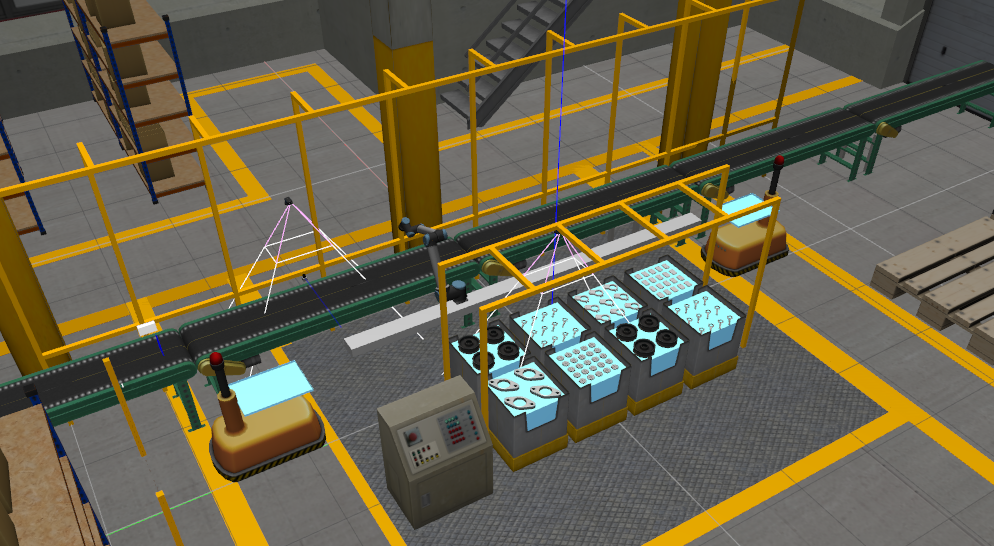
\includegraphics[width=0.7\textwidth]{ariac01.png}
	\caption{Escenario de la competición ARIAC.}
	\label{fig:ariac01}
\end{figure}

El objetivo de dicha competición es resolver una serie de problemas dentro del escenario proporcionado. En la Figura \ref{fig:ariac01} podemos observar el escenario donde los participantes realizarán las pruebas. Consta de un brazo manipulador ur10 (\textit{Figura \ref{fig:ur10}}) situado sobre un carril que le permite desplazarse, cámaras situadas en las zonas importantes, de una cinta transportadora a un lado del robot y de diversas bandejas al otro. El objetivo de las pruebas es recoger los objetos que aparecen en dicha cinta transportadora y depositarlos en la bandeja correspondiente, según las instrucciones de cada prueba. La competición consta de tres fases clasificatorias y una final que tendrá lugar en el mes de Junio de 2017.

En este proyecto nos servimos del entorno y del propio brazo robótico para desarrollar nuestros propios plugins para entender y controlar el brazo por medio de ROS.


\section{Qt}
\label{sec:plat_qt}

Qt\cite{qt} es un framework multiplataforma orientado a objetos ampliamente usado para desarrollar programas (software) que utilicen interfaz gráfica de usuario, así como también diferentes tipos de herramientas para la línea de comandos y consolas para servidores que no necesitan una interfaz gráfica de usuario.

Qt es desarrollada como un software libre y de código abierto a través de Qt Project, donde participa tanto la comunidad, como desarrolladores de Nokia, Digia y otras empresas. Qt de distribuye bajo los términos de licencias como GNU Lesser General Public License. 

Utiliza el lenguaje de programación C++ de forma nativa, aunque se pueden utilizar otros lenguajes de programación como Python añadiéndolos a través de bindings. Funciona en las principales plataformas y tiene un amplio apoyo. El API de la biblioteca cuenta con métodos para acceder a bases de datos mediante SQL, así como uso de XML, gestión de hilos, soporte de red, una API multiplataforma unificada para la manipulación de archivos y una multitud de otros métodos para el manejo de ficheros, además de estructuras de datos tradicionales.


















